
\begin{frame}{The basic problem}

%\adjincludegraphics[width=0.9\textwidth,trim={0 {.5\height} 0 0 }, clip]{static_figures/survey_and_voting.jpg}

We have a survey population, for whom we observe:
%
\begin{itemize}
 \item Covariates $\x$ (e.g.~race, gender, zip code, age, education level)
 \item Responses $\y$ (e.g.~A binary response to ``do you support Trump'')
\end{itemize}
%

We want the average response in a target population,
in which we observe only covariates.


\splitpage{
    \centering
    \only<1>{
    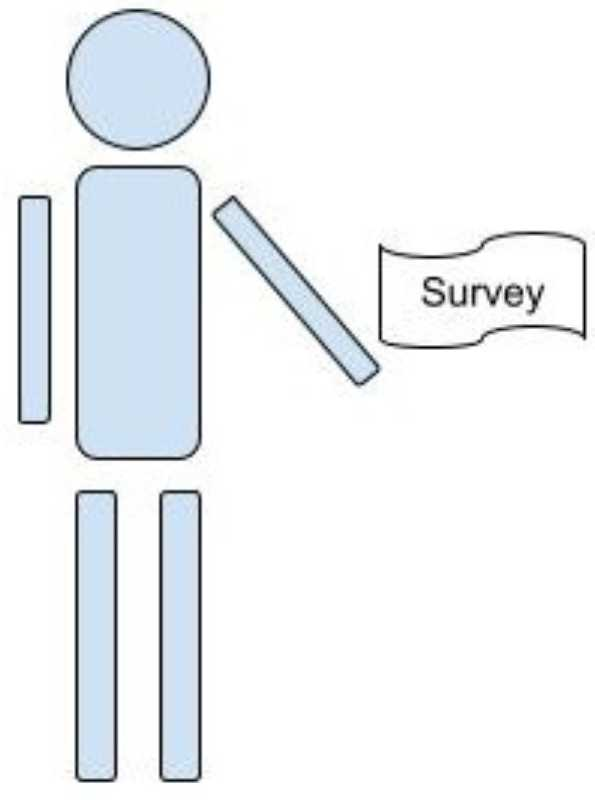
\includegraphics[width=0.5\textwidth]{static_figures/survey_man.jpg}
    }
    \only<2->{
    
\includegraphics[width=0.5\textwidth]{static_figures/survey_crazy_man.jpg}
    }
}{
    \centering
    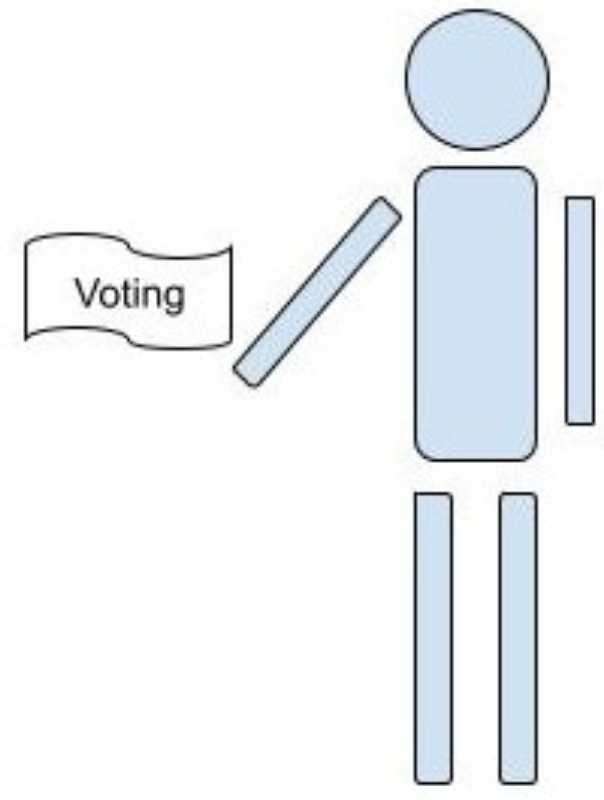
\includegraphics[width=0.5\textwidth]{static_figures/voting_man.jpg}
}

\splitpage{
    \centering
    Observe \surcol{$(\x_i, y_i)$ for $i = 1, \ldots, \nsur$}\\
}{
    \centering
    Observe \tarcol{$\x_j$ for $j = 1, \ldots, \ntar$}\\
}

\onslide<2->{
\textbf{The problem is that the populations may be very different.}
}

\onslide<3->{
    Our survey results may be biased.

    How can we use the covariates
    to say something about the target responses?
}
%
\end{frame}

%%%%%%%%%%%%%%%%%%%%%%%%%%%%%%%%%%%%%%%%%%%%%%%%%%%%%%%
%%%%%%%%%%%%%%%%%%%%%%%%%%%%%%%%%%%%%%%%%%%%%%%%%%%%%%%
%%%%%%%%%%%%%%%%%%%%%%%%%%%%%%%%%%%%%%%%%%%%%%%%%%%%%%%

\begin{frame}[t]{Two approaches}

We want $\tarcol{\mu := \meantar \y_j}$,
but don't observe target population $\tarcol{\y_j}$.

\begin{itemize}
    \item Assume $p(y | \x)$ is the same in both populations,
    \item But the distribution of $\x$ may be different in the survey and target.
\end{itemize}
%
\pause

\splitpagenoline{
    \centering
    \textbf{Calibration weighting}
}{
    \centering
    \textbf{Bayesian hierarchical modeling (MrP)}
}
%
%\\\hrulefill\\
\\[1em]
%
\splitpagenoline{
    \centering
    $\blacktriangleright$
    Choose ``calibration weights'' \surcol{$w_i$}\\
    using only the regressors $\x$\\
    (e.g.~raking weights)
}{
    \centering
    $\blacktriangleright$
    Choose $\expect{}{\y \vert \x, \theta} = m(\theta^\trans \x)$,\\
    choose prior $\p(\theta | \Sigma) \p(\Sigma)$\\
    (e.g.~Hierarchical logistic regression)
} \pause
%
\\[1em]
\splitpagenoline{
    \centering
    $\blacktriangleright$ Take
    $\surcol{\muhat_{\cal} = \meansur w_i y_i}$
}{
    \centering
    $\blacktriangleright$ Take
    $\tarcol{\yhat_j} =
        \expect{\postsur}{\y | \tarcol{\x_j}}$ and\\
    $\surcol{\muhat_{\mrp}} = \tarcol{\meantar \yhat_j}$
}\pause
%
\\[1em]
\splitpagenoline{
    \centering
    $\blacktriangleright$ Dependence of \surcol{$\muhat_{\cal}$} on \surcol{$\y_i$} is clear\\
    % (\surcol{$\w_i$} typically chosen using only $\x$)
}{
    \centering
    $\blacktriangleright$ Dependence of $\muhat_\mrp$ on \surcol{$\y_i$} very complicated\\
    (Typically via MCMC draws from $\postsur$)
}\pause
%
\\[1em]
\splitpagenoline{
    \centering
    $\blacktriangleright$ Weights give interpretable diagnostics:
    %
    \begin{itemize}
        \item Frequentist variability
        \item Partial pooling
        \item Regressor balance
    \end{itemize}
    %
}{
    \centering
    $\blacktriangleright$ \textbf{Black box}\\
    \pause
    $\leftarrow$ (We open this box, providing analogues of all these diagnostics)
}


\end{frame}


%%%%%%%%%%%%%%%%%%%%%%%%%%%%%%%%%%%%%%%%%%%%%%%%%%%%%%%
%%%%%%%%%%%%%%%%%%%%%%%%%%%%%%%%%%%%%%%%%%%%%%%%%%%%%%%
%%%%%%%%%%%%%%%%%%%%%%%%%%%%%%%%%%%%%%%%%%%%%%%%%%%%%%%

\begin{frame}{Prior work}

\textcite{gelman:2007:struggles} observes that MrP is a CW estimator when
one uses linear regression to form $\yhat$:
$$
\begin{aligned}
% \yhat_j ={}& \x_j^\trans \betahat  =
%     \x_j^\trans \left(\sumsur \x_i \x_i^\trans \right)^{-1} \sumsur \x_i \y_i \Rightarrow \\
\surcol{\muhat_{\mrp}} ={}& \tarcol{\meantar \yhat_j} =
\tarcol{\meantar \x_j^\trans} \surcol{\betahat} =
\surcol{\sumsur}
\underbrace{
\left(\tarcol{\meantar \x_j^\trans}
    \surcol{
        \left(\sum_{i'=1}^{\Nsur} \x_{i'} \x_{i'}^\trans \right)^{-1} \x_i
    }
\right)
}_{\surcol{\w^\mrp_i}}  \surcol{\y_i} \\
\end{aligned}
$$

Most existing literature on comparing CW and MrP focus on such linear models.
\footnote{
    For example,
    \textcite{gelman:2007:struggles,benmichael:2021:multilevel,chattopadhyay:2023:implied}.}

\onslide<2->{
But what if you use a non--linear link function?  Or a hierarchical model?
\vspace{1em}
\hrulefill
\begin{displayquote}
``It would also be desirable to use nonlinear methods such as regression trees ...
but then it would seem difficult to construct
even approximately equivalent weights.  Weighting and fully nonlinear models
would seem to be completely incompatible methods.''
--- \parencite{gelman:2007:strugglesrejoinder}
\end{displayquote}
}
 \onslide<3->{
\vspace{-2.5em}
\begin{block}{Our approach}
For nonlinear models, we will \textit{define}
\surcol{$\w^\mrp_i = \frac{\partial \muhat_{\mrp}}{\partial \y_i}$}.

Our primary task is then to \textbf{rigorously justify} such weights' use in common diagnostics.
\end{block}
}

\end{frame}

%%%%%%%%%%%%%%%%%%%%%%%%%%%%%%%%%%%%%%%%%%%%%%%%%%%%%%%
%%%%%%%%%%%%%%%%%%%%%%%%%%%%%%%%%%%%%%%%%%%%%%%%%%%%%%%
%%%%%%%%%%%%%%%%%%%%%%%%%%%%%%%%%%%%%%%%%%%%%%%%%%%%%%%

\begin{frame}{The weights can look very different!}

    \centering
    Does this mean anything?  Are the differences important?

    \WeightPlot{}
\end{frame}

%%%%%%%%%%%%%%%%%%%%%%%%%%%%%%%%%%%%%%%%%%%%%%%%%%%%%%%
%%%%%%%%%%%%%%%%%%%%%%%%%%%%%%%%%%%%%%%%%%%%%%%%%%%%%%%
%%%%%%%%%%%%%%%%%%%%%%%%%%%%%%%%%%%%%%%%%%%%%%%%%%%%%%%

\begin{frame}[t]{What are we weighting for?\footnote{Pun attributable to \textcite{solon:2015:weightingfor}}}


We want:
$$
\tarcol{\textrm{Target average response} =
\meantar \y_j} \approx \surcol{\meansur \w_i \y_i
= \textrm{Weighted survey average response }}
$$
We can't check this, because we don't observe $\tarcol{\y_j}$.  \pause But we can check whether:
$$
% \textrm{Target average regeressor} =
    \tarcol{\meantar \x_j} = \surcol{\meansur \w_i \x_i}
% =    \textrm{Weighted survey average regressor}
$$

Such weights satisfy ``covariate balance'' for $\x$.

You can check covariate balance for any calibration weighting estimator,
and any function $\f(\x)$.

\pause
Even more, covariate balance is the criterion for a popular class of calibration
weight estimators:

\begin{block}{Raking calibration weights}
% Select calibration weights to satisfy
``Raking'' selects weights that
%
\begin{itemize}
    \item Are as ``close as possible'' to some reference weights
    \item Under the constraint that they balance some selected regressors.
\end{itemize}
%
% $$
% \begin{aligned}
%     \textrm{ Take }
%     \w_1, \ldots, \w_{\Nsur} :={}& \argmin \sumsur (\w_s - \w_s^{\mathrm{ref}})^2 \\
%     \textrm{Subject to }
%     \meantar f(\x_p) ={}& \meansur \w_s f(\x_s)
%     \textrm{ for some function }f(\cdot).
% \end{aligned}
% $$
\end{block}



\end{frame}




%%%%%%%%%%%%%%%%%%%%%%%%%%%%%%%%%%%%%%%%%%%%%%%%%%%%%%%
%%%%%%%%%%%%%%%%%%%%%%%%%%%%%%%%%%%%%%%%%%%%%%%%%%%%%%%
%%%%%%%%%%%%%%%%%%%%%%%%%%%%%%%%%%%%%%%%%%%%%%%%%%%%%%%

\begin{frame}[t]{Generalized covariate balance checks}

% Why would you want covariate balance?  Some commonly stated reasons:
% %
% \begin{itemize}
% \item To reduce the variance of inverse propensity weights (IPW)
% \item To check the accuracy of IPW
% \item To exactly balance ``important regressors''
% \end{itemize}
%
% Common to these motivations is the following concen:

We want to balance $f(\x)$ because we think
$\expect{}{\y \vert \x}$ might plausibly vary $\propto f(\x)$,
and want to check whether our estimator can capture this variability.
%
\only<2>{
\begin{block}{Balance--informed sensitivity check (BISC) (informal)}
    Pick a small $\delta$, and define a \emph{new response variable} $\ytil$ such that
    $$
    \expect{}{\ytil \vert \x} = \expect{}{\y \vert \x} + \delta f(\x).
    $$
    We know the change this is supposed to induce in the target population.\\[1em]

    Covariate balance checks whether our estimators produce the same change.
    %
\end{block}
}
%
\only<3->{
\begin{block}{Balance--informed sensitivity check (BISC) (formal)}
    Pick a small $\delta$, and define a \emph{new response variable} $\ytil$ such that
    $$
    \expect{}{\ytil \vert \x} = \expect{}{\y \vert \x} + \delta f(\x).
    $$
    We know the expected change this perturbation produces in the target distribution:
    $$
    \begin{aligned}
        \tarcol{
            \expect{}{\mu(\ytil) - \mu(\y) | \x} =
            \meantar \left(\expect{}{\ytil | \x_p} - \expect{}{\y | \x_p}\right) =
            \delta \meantar f(\x_j)}
    \end{aligned}
    $$
    Then, check whether your estimator $\muhat(\cdot)$ produces
    the same change for observed \surcol{$\ytil, \y$}:
    $$
    \begin{aligned}
        \underbrace{
        \surcol{\muhat(\ytil) - \muhat(\y)}
        }_{
            \substack{
                \text{Replace weighted averages} \\
                \text{with changes in an estimator}
            }
        }
        \overset{\textrm{check}}{\approx}
        \tarcol{
        \delta \meantar f(\x_j).}
    \end{aligned}
    $$
\end{block}
}

\onslide<4->{
    When $\muhat(\cdot) = \muhat_\cal(\cdot)$,
    BISC recovers the standard covariate balance check. \\[1em]
    When $\muhat(\cdot) = \muhat_\mrp(\cdot)$ and $\delta$ is small,
    BISC recovers our proposal. \\[1em]
}

\end{frame}


